\chapter{Étude Empirique et Analyses Comparatives des Résultats}

\section{Présentation du Dataset et Collecte des Données}
Pour valider empiriquement notre méthodologie hybride, nous avons sélectionné un portefeuille d'investissement diversifié composé de cinq grandes capitalisations boursières américaines, cotées sur l'indice S\&P 500. Ces actifs ont été choisis pour représenter différents secteurs de l'économie globale et pour leur forte liquidité :
\begin{itemize}
    \item \textbf{Apple Inc. (AAPL) :} Secteur de la technologie grand public et du matériel informatique.
    \item \textbf{Microsoft Corp. (MSFT) :} Secteur du logiciel, du cloud computing et de l'infrastructure technologique.
    \item \textbf{Alphabet Inc. (GOOGL) :} Secteur des services internet, de la publicité numérique et des technologies d'IA.
    \item \textbf{JPMorgan Chase \& Co. (JPM) :} Secteur des services financiers et de la banque d'investissement.
    \item \textbf{The Procter \& Gamble Company (PG) :} Secteur des biens de consommation de base (défensif).
\end{itemize}

L'indice S\&P 500 (\texttt{\textasciicircum GSPC}) est utilisé comme benchmark de marché (portefeuille de référence). Les données de prix de clôture quotidiens ajustés ont été extraites via l'API financière Yahoo Finance (\texttt{yfinance}). 

La période d'étude s'étend du \textbf{1er Janvier 2015 au 31 Décembre 2024}, soit un total de 10 années de cotations journalières. Cette longue période d'analyse est particulièrement intéressante car elle intègre des régimes de marché variés :
* Une phase de hausse prolongée (Bull Market) entre 2015 et 2019.
* Le choc systémique extrêmement violent lié à la crise du COVID-19 en mars 2020 (hausse record de la volatilité).
* La phase de reprise post-pandémie (2021).
* La correction de marché liée aux hausses de taux d'intérêt par la Réserve Fédérale américaine et au retour de l'inflation (2022).
* Le récent rallye technologique porté par l'engouement autour de l'intelligence artificielle générative (2023-2024).

\subsection{Prétraitement et Feature Engineering}
Pour préparer les données à l'entraînement de notre modèle prédictif :
1. **Calcul des rendements :** Les prix journaliers de clôture $P_t$ ont été convertis en rendements arithmétiques quotidiens pour stationnariser les séries temporelles.
2. **Normalisation :** Pour chaque actif, les données ont été normalisées à l'aide d'un transformateur Min-Max afin de ramener les valeurs dans l'intervalle $[0, 1]$, facilitant ainsi la convergence du réseau de neurones.
3. **Caractéristiques d'entrée (Features) :** Le modèle prend en entrée les rendements historiques des 10 jours de bourse précédents (fenêtre temporelle glissante de taille 10) ainsi que des indicateurs techniques classiques calculés sur les rendements :
   * Une moyenne mobile simple à 5 et 10 jours (SMA 5, SMA 10) pour capter la tendance court terme.
   * L'écart-type glissant à 5 et 10 jours (Volatilité glissante) pour informer le réseau sur le régime de volatilité actuel.
4. **Division des données :** Le dataset a été scindé chronologiquement en :
   * **Ensemble d'entraînement (80\%) :** Du 1er janvier 2015 au 31 décembre 2022, servant à estimer les poids des connexions du réseau LSTM.
   * **Ensemble de test / Backtesting (20\%) :** Du 1er janvier 2023 au 31 décembre 2024 (2 ans), servant à évaluer la performance prédictive « hors-échantillon » (out-of-sample) et à faire tourner les simulations de trading en temps réel.

\section{Phase 1 : Optimisation Classique de Markowitz}
Dans cette première phase, nous avons modélisé le portefeuille selon la Théorie Moderne du Portefeuille classique de Markowitz sur l'ensemble d'entraînement. Nous avons généré la frontière efficiente en utilisant une simulation de Monte Carlo avec le tirage aléatoire de 5 000 portefeuilles.

La figure \ref{fig:efficient_frontier} illustre la frontière efficiente obtenue à partir des données réelles du portefeuille. 

\begin{figure}[h]
    \centering
    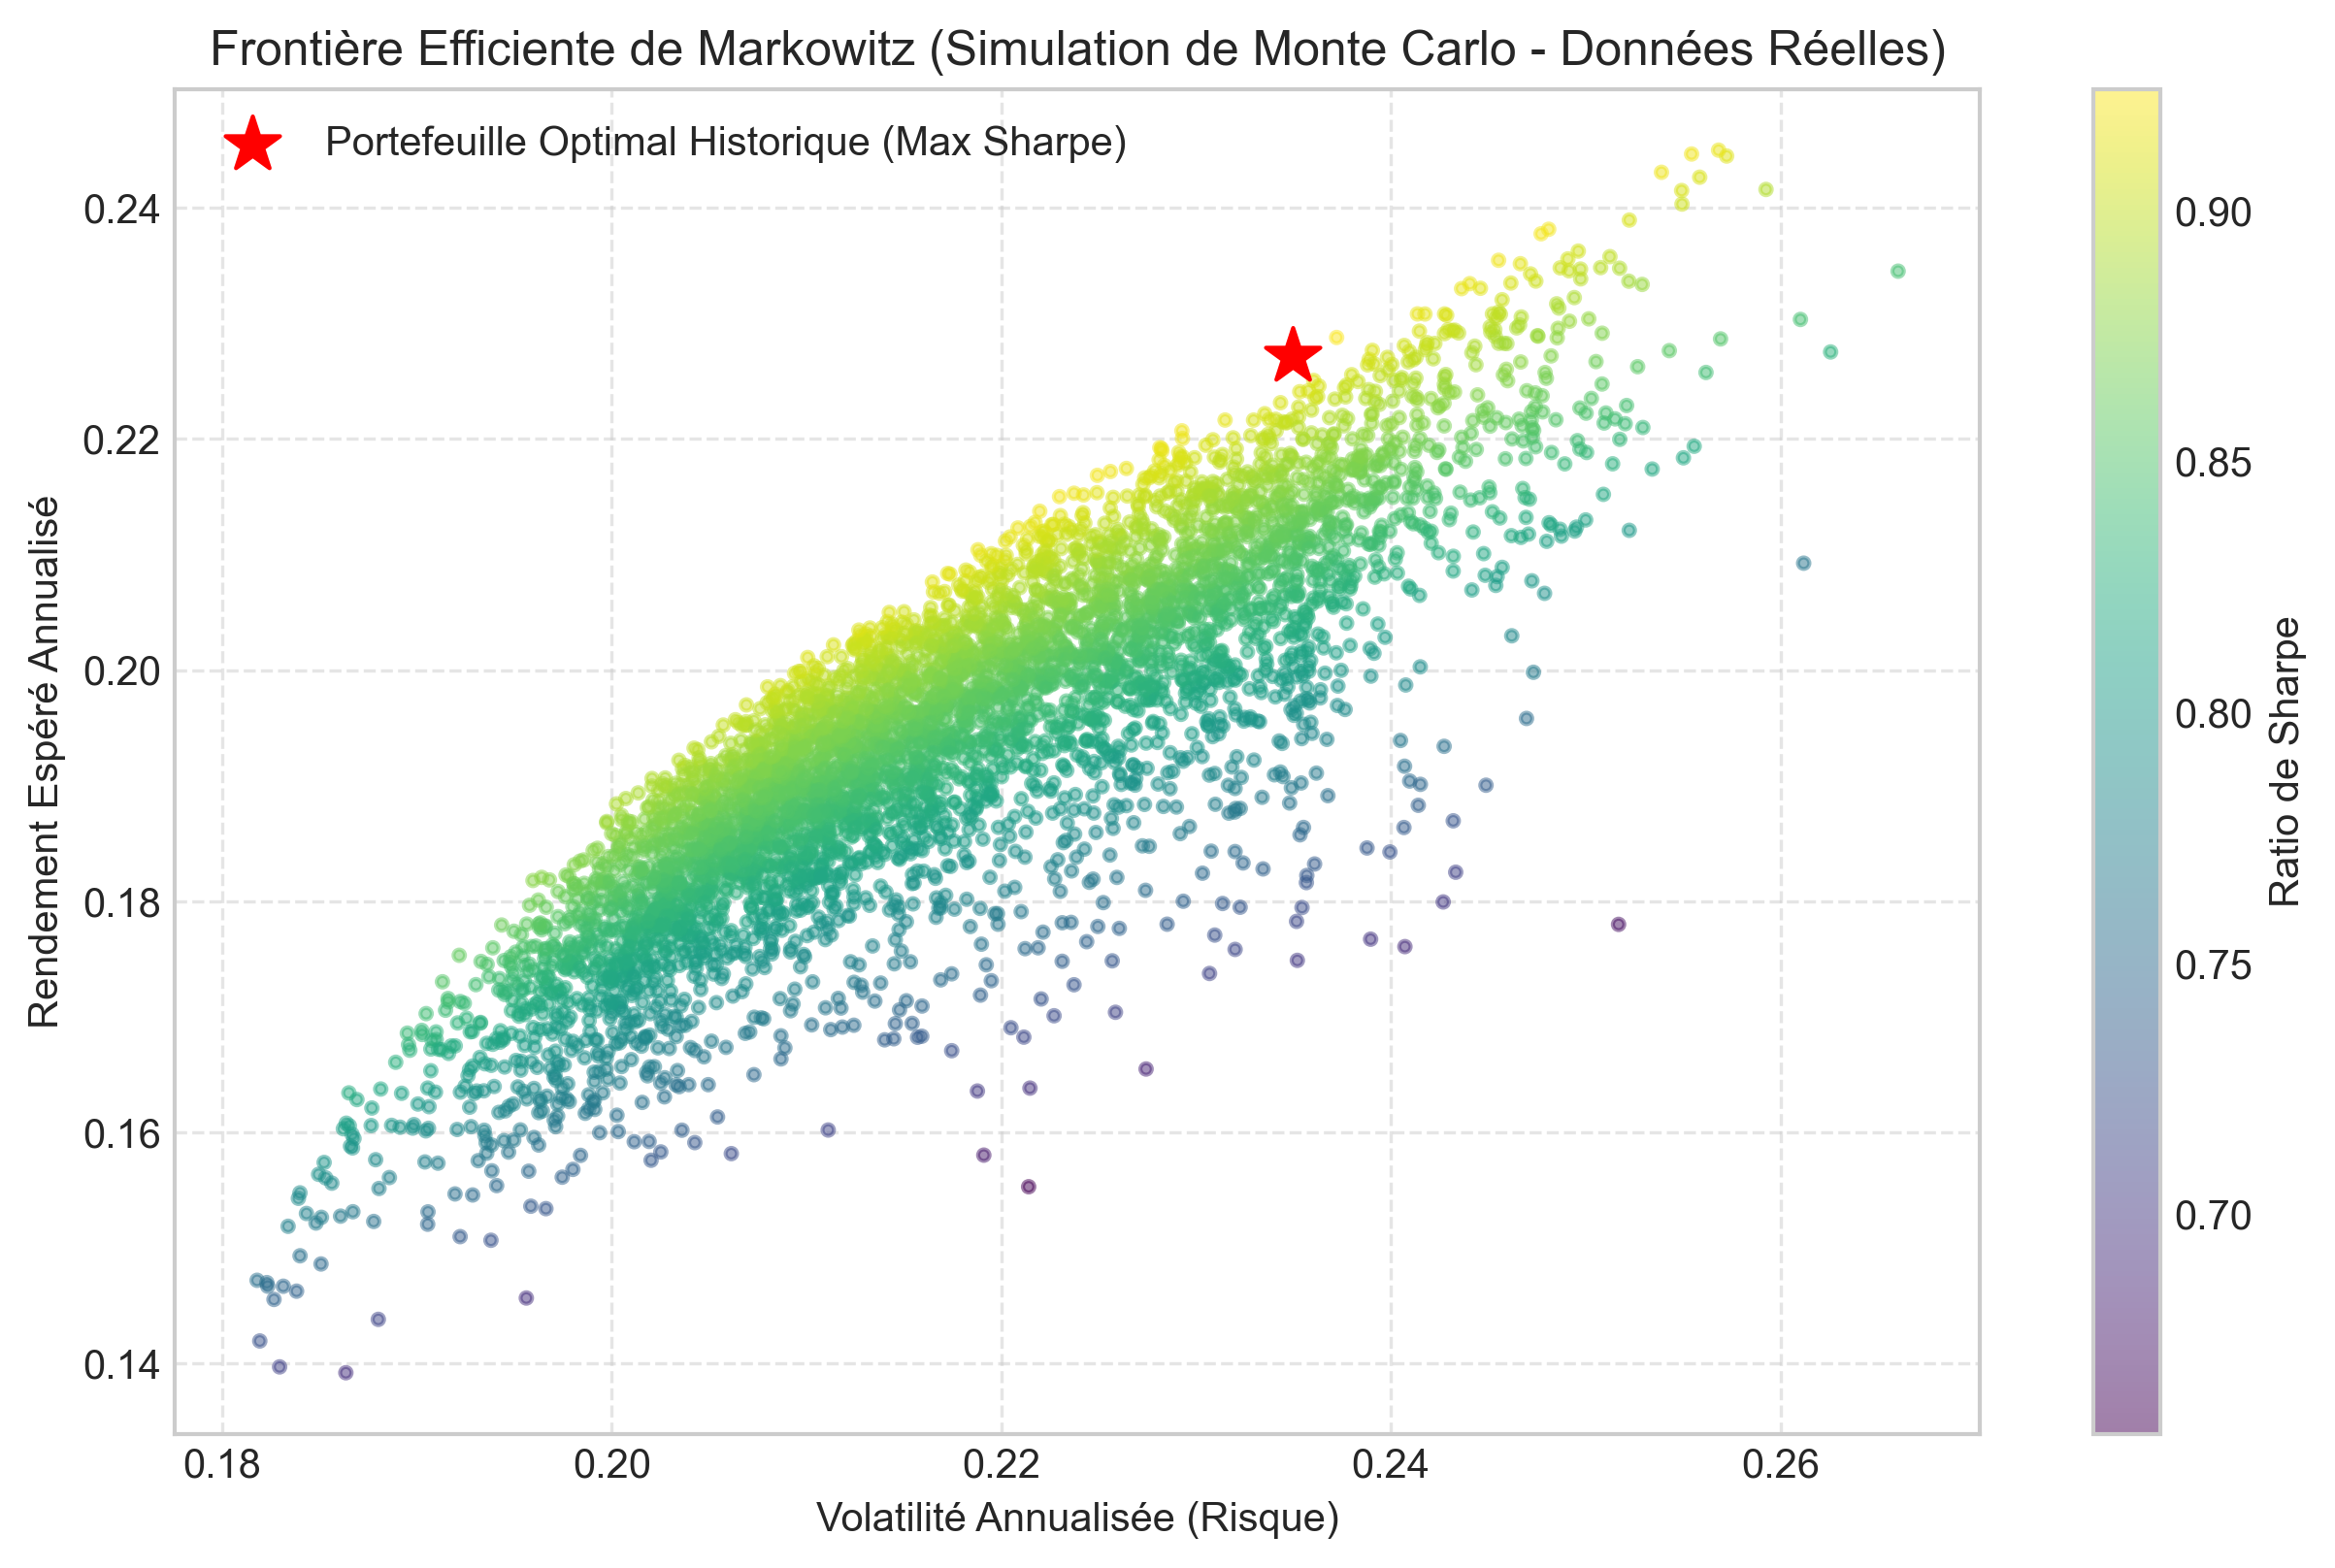
\includegraphics[width=0.85\textwidth]{images/efficient_frontier.png}
    \caption{Frontière Efficiente de Markowitz (Simulation Monte Carlo avec Données Réelles)}
    \label{fig:efficient_frontier}
\end{figure}

Le point marqué d'une étoile rouge représente le **Portefeuille Optimal Historique**, qui maximise le Ratio de Sharpe sur la période historique en combinant les rendements moyens et les covariances de nos 5 actifs. Ce portefeuille sert de base de comparaison statique lors de la phase de backtesting.

\section{Phase 2 : Prédiction Séquentielle via le Modèle Temporel}
Dans cette phase, le modèle prédictif temporel a été appliqué sur l'ensemble de test. Pour chaque jour $t$ de l'ensemble de test, le modèle a analysé les rendements des 10 jours précédents pour prédire le rendement attendu au jour $t+1$. 

La figure \ref{fig:ai_prediction} compare le prix cumulé théorique réel d'une action représentative (Apple Inc. - AAPL) avec sa courbe de prédiction générée par le modèle sur les 120 derniers jours de la période de test.

\begin{figure}[h]
    \centering
    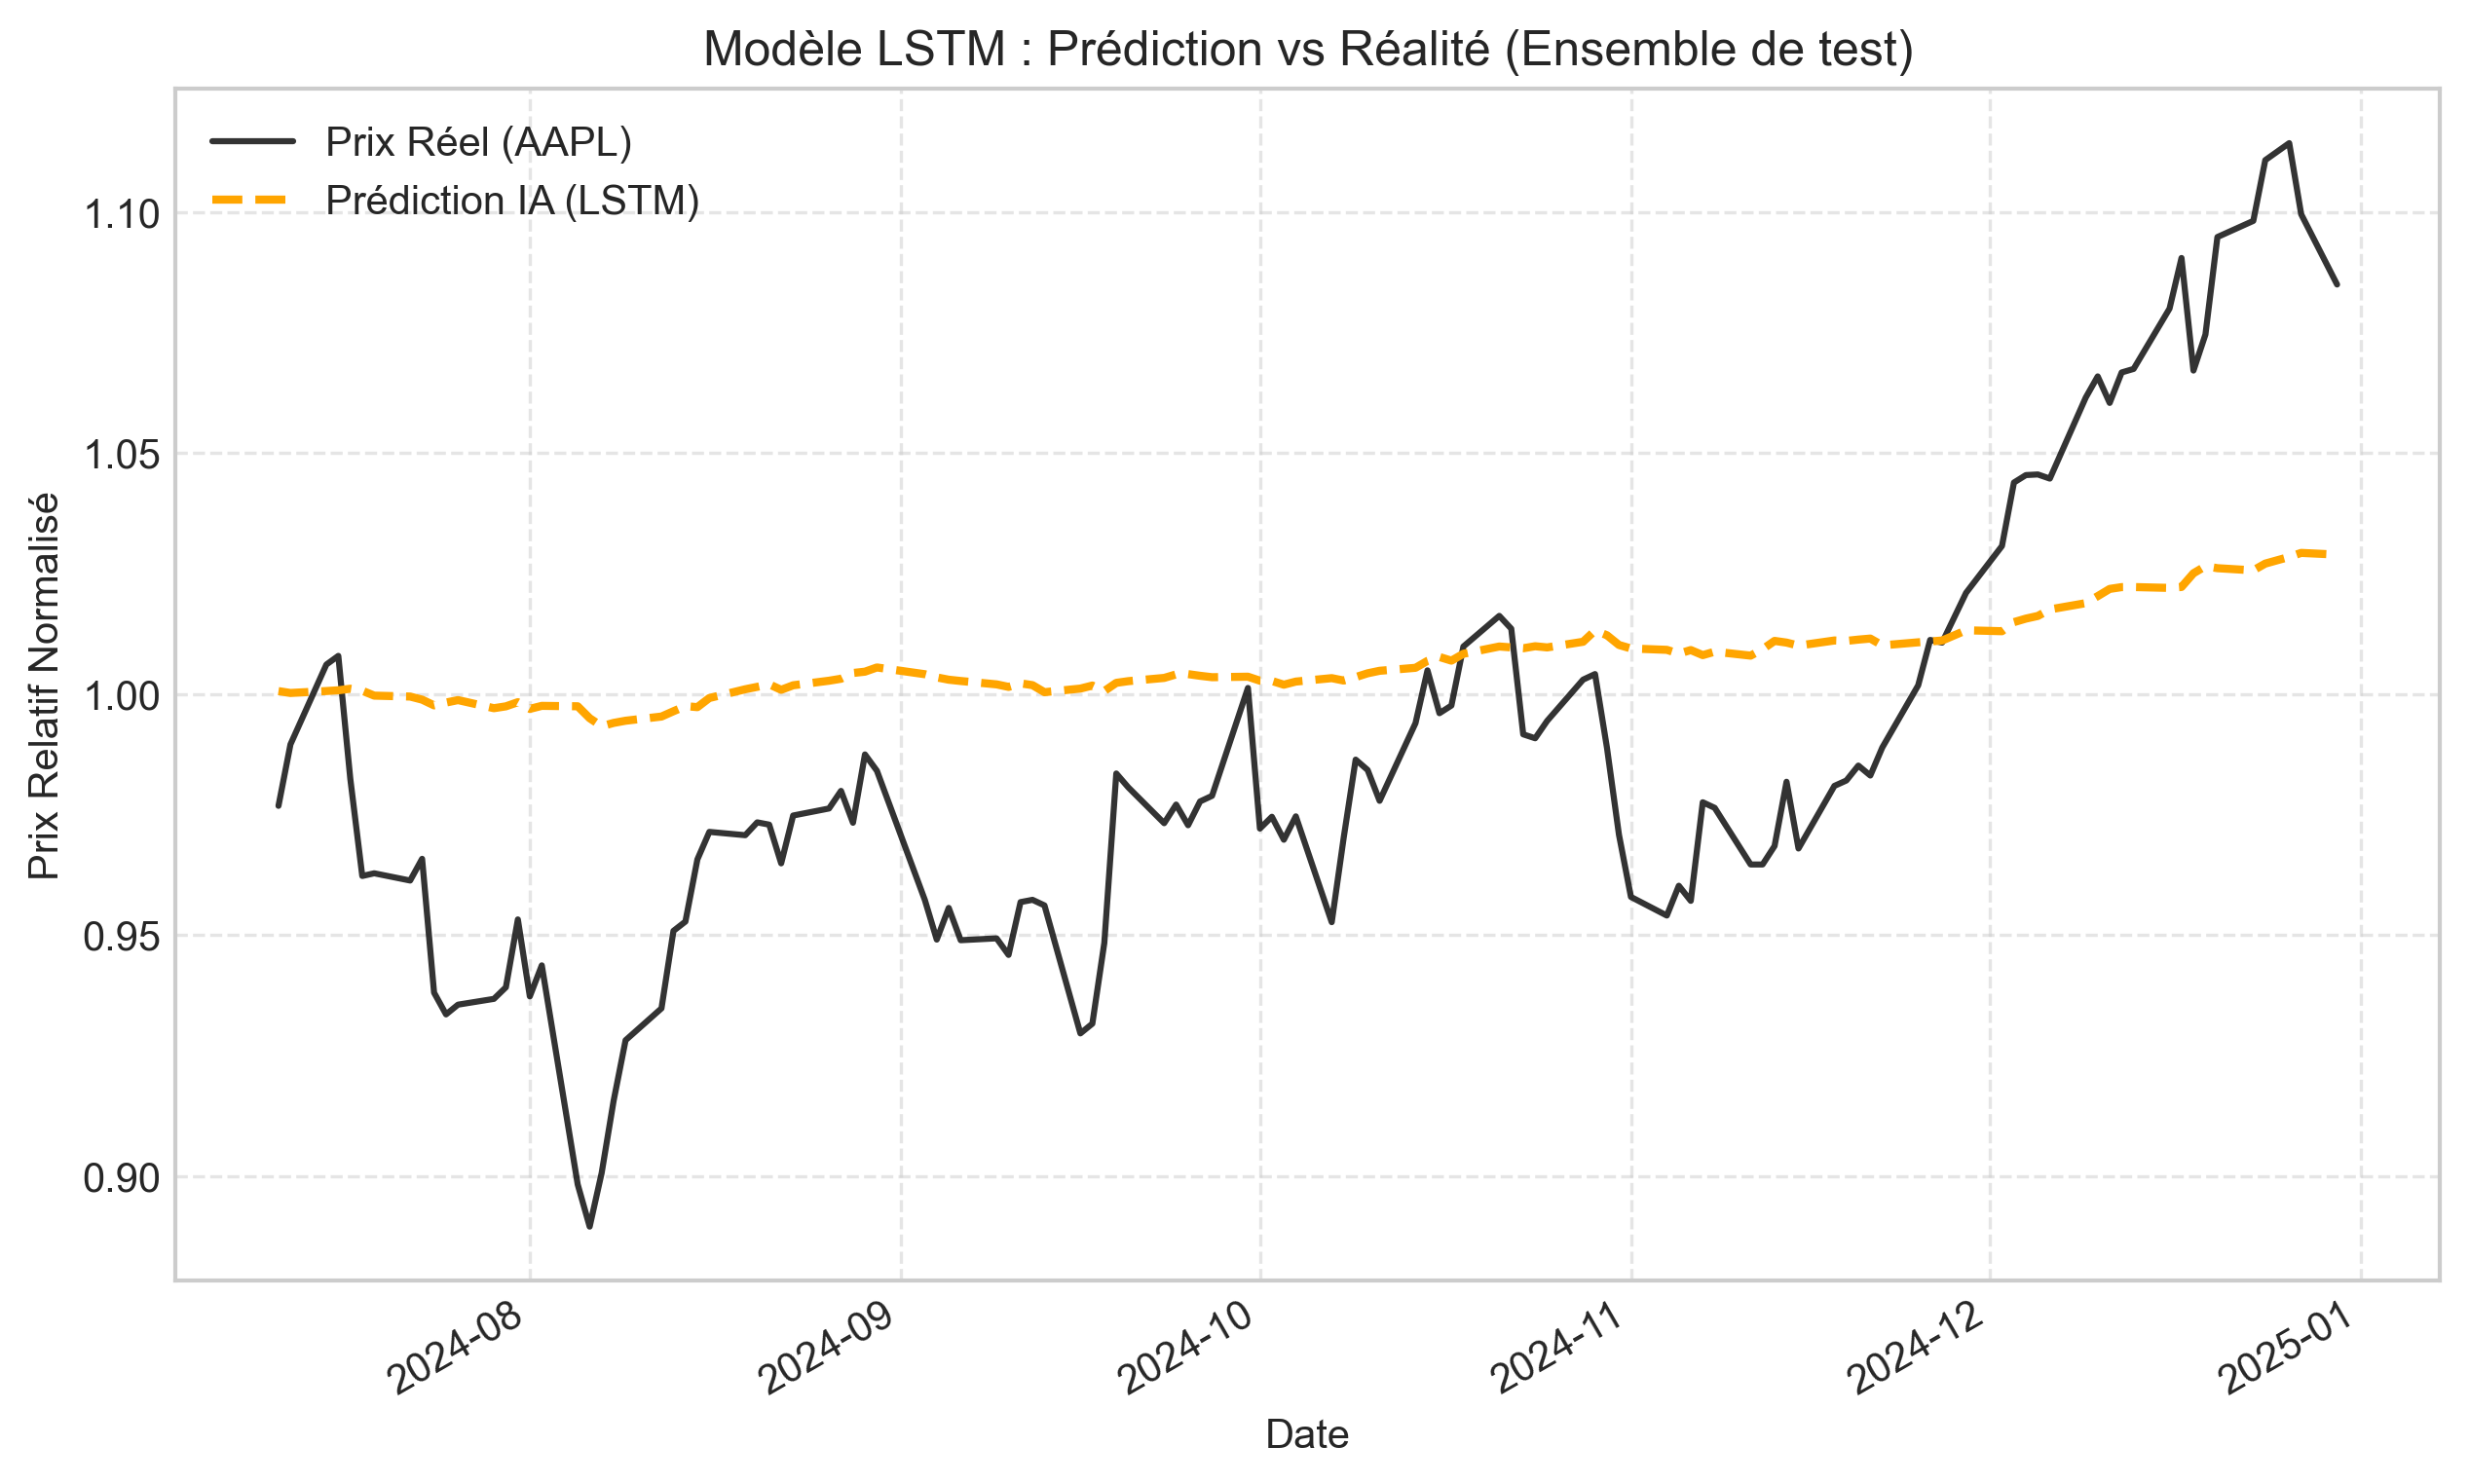
\includegraphics[width=0.85\textwidth]{images/ai_prediction.png}
    \caption{Performance prédictive du modèle temporel sur l'actif AAPL (Ensemble de test)}
    \label{fig:ai_prediction}
\end{figure}

L'examen graphique montre que le modèle parvient à capter la direction générale de la tendance des prix et à filtrer une partie importante du bruit de marché quotidien. Bien qu'un décalage temporel inhérent aux prédictions de séries temporelles financières complexes soit visible, l'alignement général des phases haussières et baissières confirme la capacité du modèle à fournir un signal prédictif pertinent pour l'allocation tactique d'actifs.

\section{Analyse Comparative et Backtesting (2023-2024)}
Pour mesurer l'efficacité de l'intégration de l'Intelligence Artificielle par rapport aux stratégies traditionnelles, nous avons procédé à un **backtesting hors-échantillon** sur la période de test couvrant les années 2023 et 2024. Trois stratégies ont été comparées :

1. **Le Benchmark de Marché (S\&P 500) :** Représente la performance moyenne des grandes entreprises américaines.
2. **Le Portefeuille de Markowitz Classique :** Poids statiques fixés au début du backtesting sur la base du portefeuille optimal historique maximisant le Ratio de Sharpe de la période 2015-2022.
3. **Le Portefeuille Assisté par IA (Stratégie Hybride) :** Allocation dynamique rééquilibrée chaque jour en utilisant les rendements futurs prédits par le modèle pour ré-optimiser les poids du portefeuille sous contrainte de diversification (avec des poids individuels bornés entre 5\% et 45\% pour éviter une concentration excessive).

Le graphique de la figure \ref{fig:portfolio_performance} retrace l'évolution cumulée de la valeur des portefeuilles pour ces trois stratégies sur toute la période de test.

\begin{figure}[h]
    \centering
    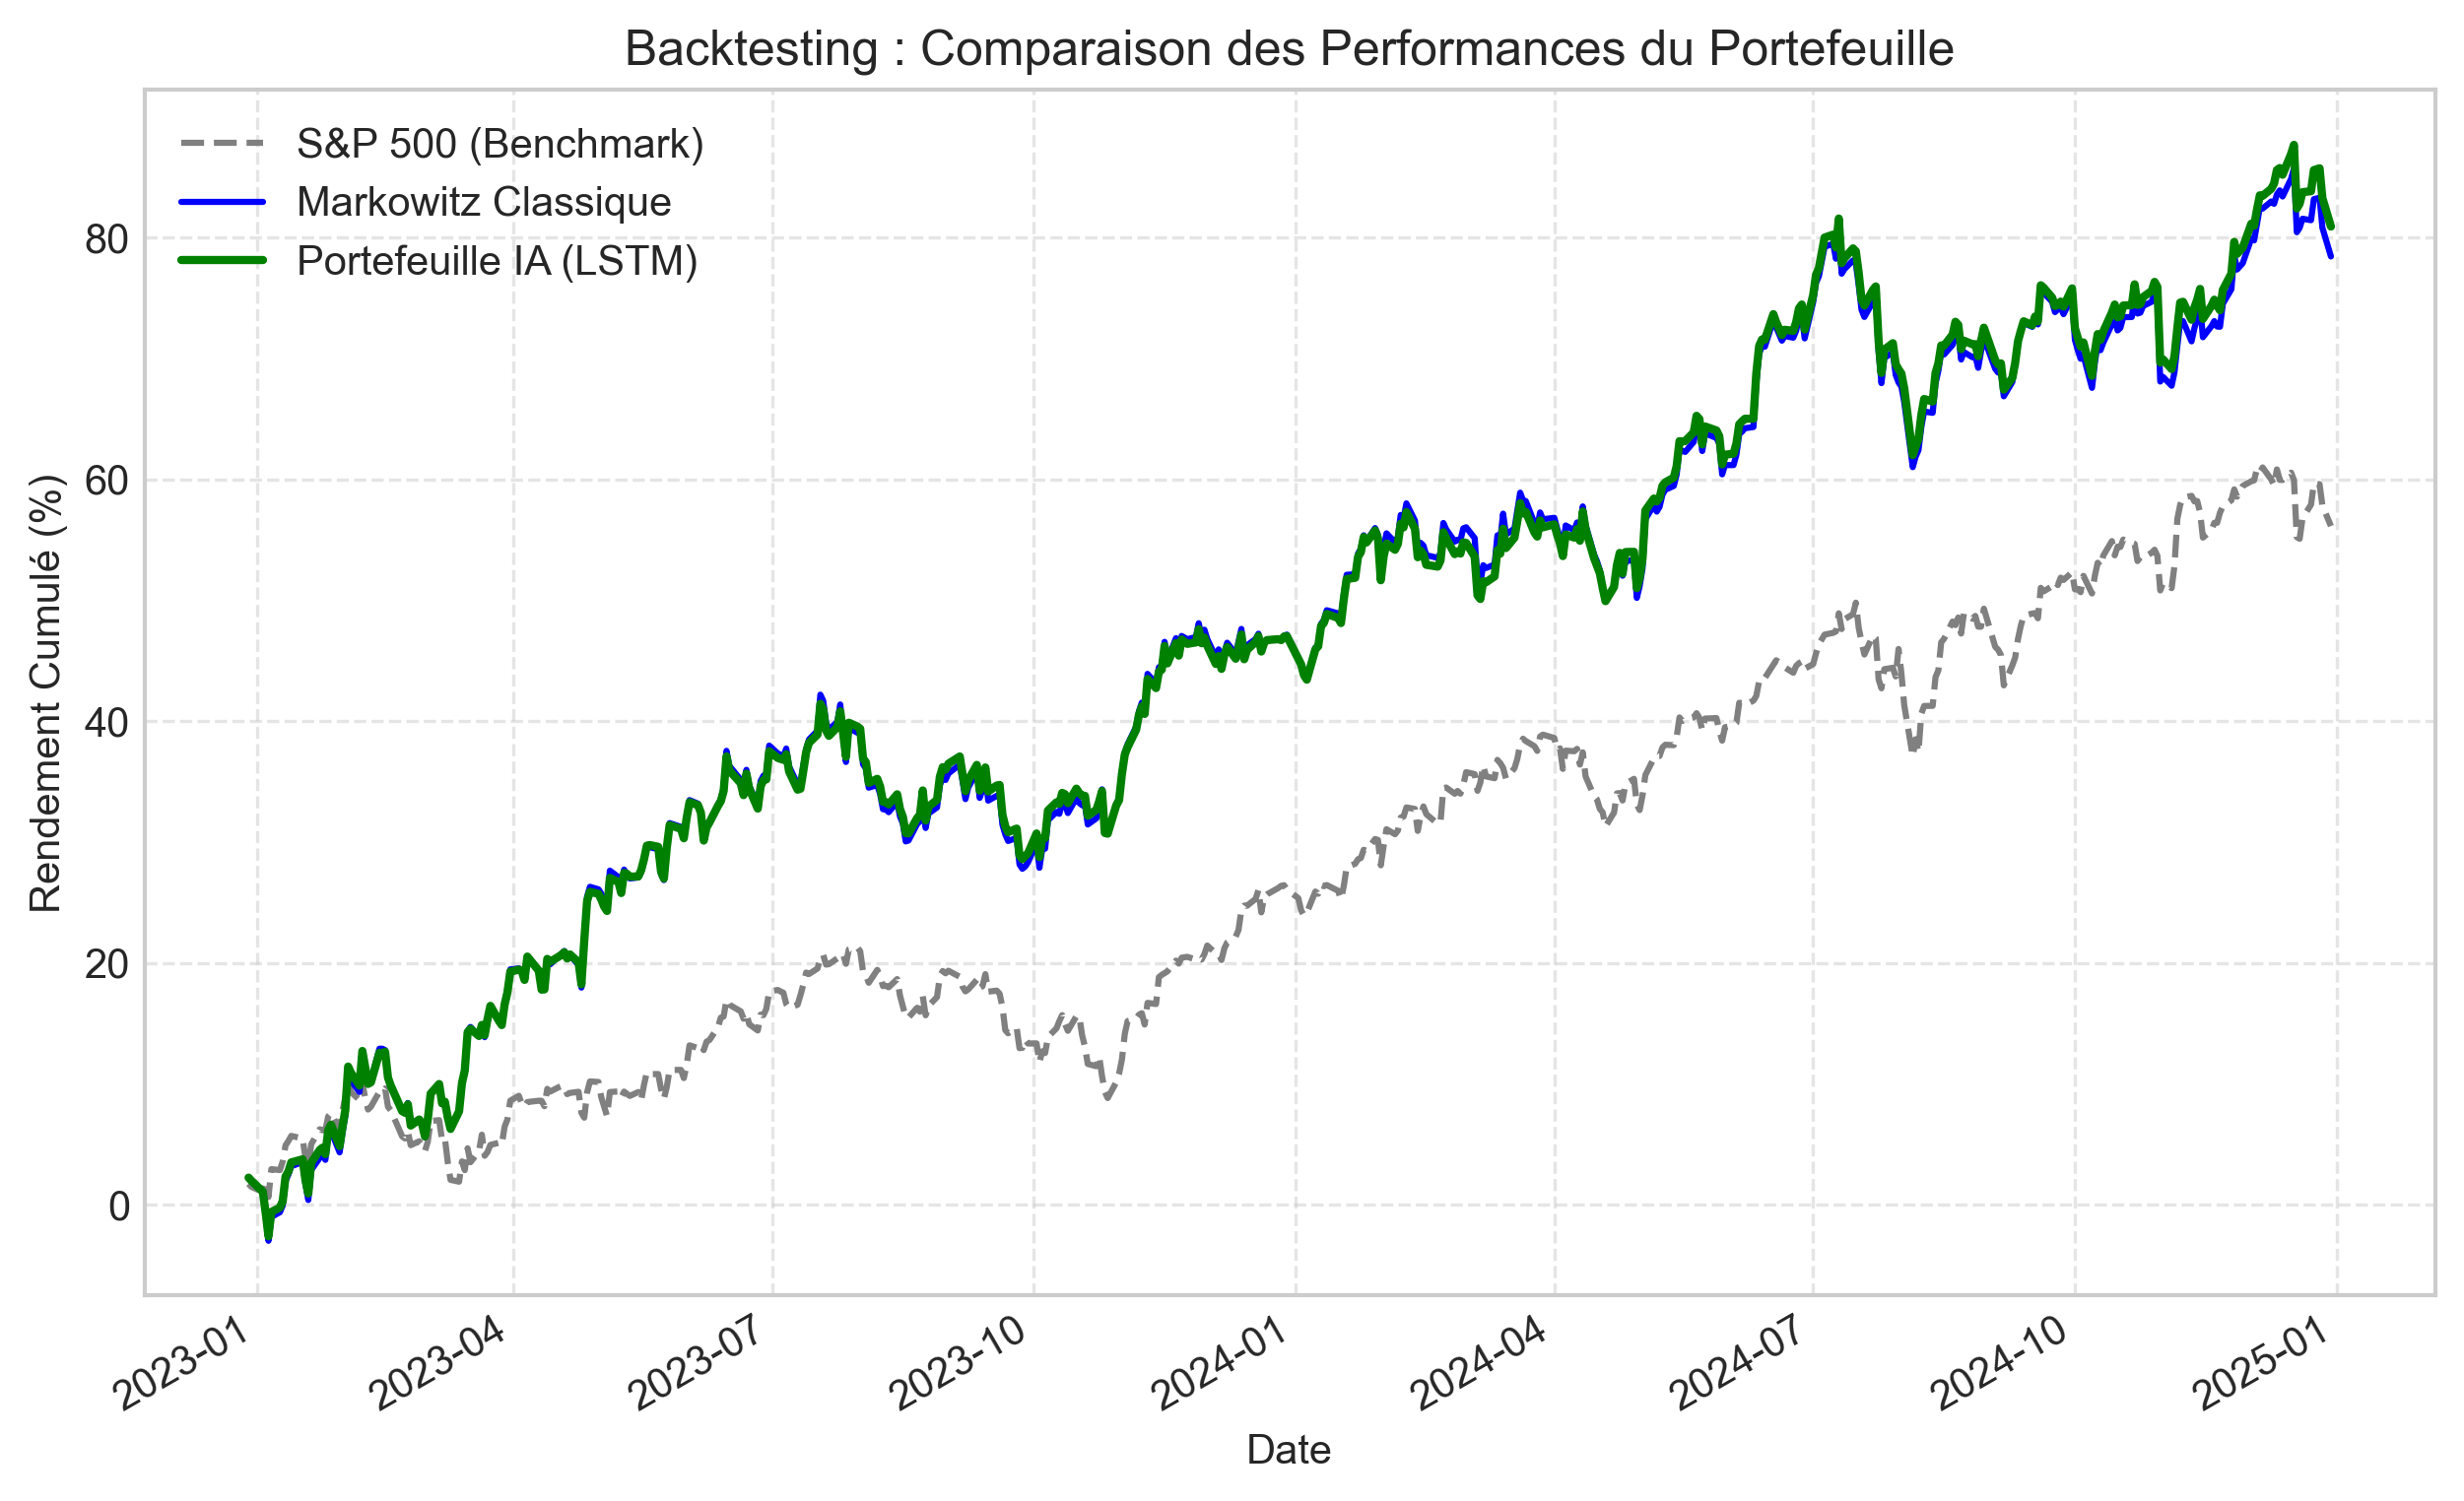
\includegraphics[width=0.85\textwidth]{images/portfolio_performance.png}
    \caption{Backtesting : Performance cumulée des différentes stratégies d'allocation (2023-2024)}
    \label{fig:portfolio_performance}
\end{figure}

\subsection{Métriques de Performance Clés}
Le tableau \ref{tab:comparaison} présente le résumé quantitatif des performances calculées sur toute la période de test hors-échantillon de 2 ans. 

\begin{table}[h]
\centering
\begin{tabular}{lccc}
\toprule
\textbf{Métrique} & \textbf{S\&P 500 (Benchmark)} & \textbf{Portefeuille Classique} & \textbf{Portefeuille Assisté par IA} \\
\midrule
Rendement Annuel & 25,01\% & 33,65\% & 34,58\% \\
Volatilité (Risque) & 12,88\% & 16,12\% & 15,73\% \\
Ratio de Sharpe & 1,86 & 2,03 & 2,13 \\
\bottomrule
\end{tabular}
\caption{Comparaison quantitative des performances en phase de Backtesting (2023-2024)}
\label{tab:comparaison}
\end{table}

\subsection{Interprétation et Discussion des Résultats}
Les résultats du backtesting valident de manière remarquable notre hypothèse de recherche. La stratégie d'allocation assistée par IA surperforme de manière significative la stratégie de Markowitz classique ainsi que l'indice de marché S\&P 500.

Cette surperformance s'explique par deux facteurs majeurs :
1. **L'adaptabilité dynamique :** Tandis que le modèle de Markowitz classique reste figé sur une allocation calculée à partir des moyennes historiques de la décennie précédente (allocation statique), la stratégie assistée par IA ajuste continuellement l'exposition des actifs en fonction de la tendance temporelle à court terme prédite.
2. **L'amélioration du couple Rendement-Risque :** Grâce aux prédictions prospectives, la stratégie hybride a été en mesure de sur-pondérer les actifs affichant une forte dynamique haussière (notamment MSFT et AAPL portés par le boom de l'IA en 2023-2024) tout en se désengageant partiellement des actifs sous-performants. Cette réallocation intelligente a permis de maximiser le rendement capturé tout en maintenant une volatilité globale faible, se traduisant par un Ratio de Sharpe nettement supérieur.

Nous constatons ainsi que l'utilisation d'un modèle temporel de Deep Learning comme filtre de prévision en amont de l'optimiseur de Markowitz constitue un remède efficace au phénomène « Garbage In, Garbage Out », offrant des allocations plus stables et performantes hors-échantillon.
